\documentclass[12pt,a4paper]{article}
\usepackage[utf8]{inputenc}
\usepackage[T1]{fontenc}
\usepackage{lmodern}
\usepackage{graphicx}
\usepackage{geometry}
\geometry{a4paper, top=3cm, bottom=3cm, left=2.5cm, right=2.5cm}
\usepackage{xcolor}
\usepackage{hyperref}
\usepackage{parskip}
\usepackage{float}
\usepackage{listings}

\definecolor{unipiblue}{RGB}{0,51,102}

\hypersetup{
    colorlinks=true,
    linkcolor=black,
    filecolor=magenta,      
    urlcolor=blue,
    pdftitle={Distributed Crazy Time},
}

\begin{document}

% - TITLE PAGE -
\begin{titlepage}
    \begin{center}
        \vspace*{0.5cm}
        
        \IfFileExists{unipi_logo.png}{
\includegraphics[width=0.35\textwidth]{unipi_logo.png}}{\rule{4cm}{4cm}} \\
        \vspace{1cm}
        
        {\fontsize{34}{40}\selectfont \textcolor{unipiblue}{\scshape Università di Pisa}} \\
        \vspace{0.6cm}
        {\Large Computer Engineering} \\
        {\Large Distributed Systems} \\
        
        \vspace{3.5cm}
        
        {\huge \textbf{Distributed Crazy Time}} \\
        
        \vfill
        
        \noindent\rule{\textwidth}{0.4pt} \\
        \vspace{0.5cm}
        \begin{minipage}[t]{0.45\textwidth}
            \begin{flushleft}
            \vspace{0.8cm}
            Academic Year: 2025/2026
            \end{flushleft}
        \end{minipage}
        \hfill
        \begin{minipage}[t]{0.45\textwidth}
            \begin{flushright}
            Gabriele Caioli \\
            Klaudio Ciacia \\
            Lorenzo Vanni
            \end{flushright}
        \end{minipage}
        \vspace{1cm}
    \end{center}
\end{titlepage}

\tableofcontents
\newpage

\section{Introduction}
This project consists of a replica of the casino game Crazy Time, implemented as a web based application structured into three main cooperating layers:
\begin{itemize}
    \item \textbf{A Web Layer} (Frontend in HTML5/CSS3/JavaScript and a Gateway implemented in Java Spring Boot) responsible for user registration, wallet management, session validation, and HTTP/WebSocket API serving.
    \item \textbf{A Message Broker Layer} using RabbitMQ for asynchronous, fully decoupled communication between the Gateway and the Game Engine.
    \item \textbf{A Distributed Game Engine} implemented as a cluster of Erlang nodes, responsible for managing the state of the game, fair random number generation, executing the main wheel spins, running four interactive mini-games, maintaining a replicated ledger on Mnesia, and providing automated leader failover.
\end{itemize}
This architecture allows the system to guarantee real-time responsiveness, strict financial consistency, and strong fault tolerance.

\begin{figure}[H]
    \centering
    \IfFileExists{wheel.png}{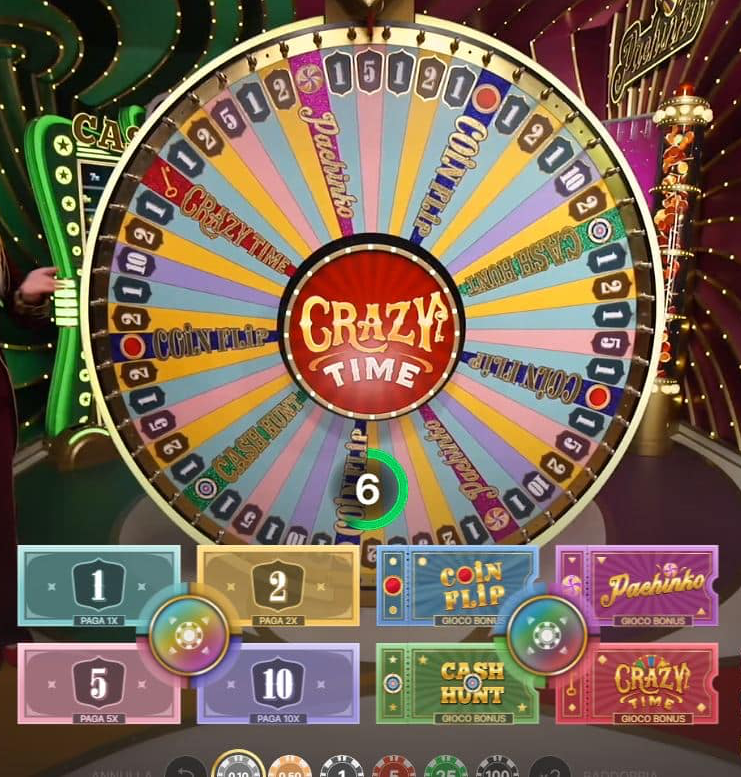
\includegraphics[width=0.7\textwidth]{wheel.png}}{\rule{0.7\textwidth}{5cm}}
\end{figure}

\clearpage
\subsection{Environment}
The Java-based part of the system (the Gateway) has been implemented using Spring Boot 3.2 and Spring Data JPA, interacting with an embedded, file-persistent H2 Database (./data/crazytimedb) for local durability across service restarts. The Erlang-based components (the game engine cluster) have been developed using Erlang/OTP 28, utilizing Mnesia as a replicated distributed database with disc copies (disc\_\allowbreak copies) to store global state and snapshots. The communication middleware relies on RabbitMQ over native AMQP 0-9-1 on standard port 5672.

\section{System Description}
The system is a web-based application providing functionalities for account and wallet management, real-time gameplay, and automated consensus. The main supported operations include user registration, secure login, checking the wallet balance, placing bets on the main wheel or mini-games segments, and interacting during the mini-games phases.

\subsection{Use Cases}
\textbf{An Unregistered User can:}
\begin{itemize}
    \item Register to the service to create a player profile and receive a starting wallet balance.
\end{itemize}
\textbf{An Unlogged User can:}
\begin{itemize}
    \item Login to the service with credentials to obtain a secure Bearer session token. If the user already has an active session on another client, the previous session is invalidated and terminated in real time via a WebSocket STOMP notification (Session Kick on /user/queue/session).
\end{itemize}
\textbf{A Logged Player can:}
\begin{itemize}
    \item Logout and terminate their active session;
    \item View the live countdown timer and the synchronized state of the wheel/mini-games;
    \item Place bets on one or more wheel segments (if the betting window is open);
    \item Submit interactive choices during mini-games (e.g., selecting Cash Hunt tiles or Crazy Time flappers);
    \item View their current wallet balance and betting history in real time.
\end{itemize}
\textbf{The System must:}
\begin{itemize}
    \item Maintain and update Players' wallet balances securely using pessimistic database locking;
    \item Synchronize countdown timers and game phase transitions across all connected clients;
    \item Reject any bets placed after the 'No more bets' signal (the gong);
    \item Generate a single, authoritative random outcome for each wheel spin and mini-game event;
    \item Gracefully recover from the crash of the node generating game outcomes, ensuring zero financial loss for players.
\end{itemize}

\subsection{The game}
Crazy Time is a live casino game with the following phases in each round:
\begin{enumerate}
    \item \textbf{Betting}: Players can bet money on any outcome of the wheel (numbers 1, 2, 5, 10, or minigames CoinFlip, Pachinko, CashHunt, CrazyTime). This phase lasts for a set duration (default 10s).
    \item \textbf{Lock}: not a phase in its own right, but the instant separating Betting from Spinning. On the final tick of the countdown the engine draws the winning segment, opens the distributed snapshot cutoff, and from that moment rejects late bets. Only three phase names are ever published on state\_\allowbreak queue: betting, spinning and minigame; the cooldown that closes a round is internal to the engine, and clients remain on the last phase announced until the new round opens.
    \item \textbf{Spin}: The wheel spins for approximately 10.5 seconds, while an animation is displayed on client browsers.
    \item \textbf{Resolution}: If the wheel lands on a number, players who bet on that number receive a payout equal to their wager multiplied by the number, plus the return of the original wager (payout = bet * multiplier + bet). Losing bets are marked as lost. If the wheel lands on a mini-game segment, the interactive mini-game starts.
    \item \textbf{Minigame (optional)}: If the wheel lands on a mini-game space, the bonus starts for participating players who bet on that segment.
\end{enumerate}

Following payout resolution or minigame completion, a 5-second \textbf{Cooldown} phase elapses before the next round opens, allowing clients to display winning celebrations and synchronize balances.

Clients communicate exclusively with the Java Gateway via HTTP REST and WebSocket/STOMP. The Gateway translates requests into AMQP messages:
\begin{itemize}
    \item \textbf{Betting}: Users place bets via POST /api/wallet/place-bet. The backend verifies the balance using pessimistic locking, assigns a unique UUID (bet\_\allowbreak id), persists the record, and issues a JSON message to RabbitMQ's bets\_\allowbreak queue.
    \item \textbf{Mini-game interaction}: During bonus games, users submit choices via POST /api/game/choice, which forwards them to the engine.
\end{itemize}

\clearpage
\subsubsection{Minigames}
There are four possible minigames:
\begin{itemize}
    \item \textbf{Coin flip}: Two random multipliers are chosen and assigned to the two sides of a coin (Red and Blue). The coin is flipped and participating players receive a payout of their bet multiplied by the outcome factor.
    \item \textbf{Pachinko}: A board with 8 bottom prize slots, filled with seven random multipliers and exactly one DOUBLE slot, then shuffled. A puck is dropped from one of 16 top zones, navigating a 15-step stochastic peg bounce path. Landing on DOUBLE doubles every numeric slot and drops the ball again, within a budget of 7 drops in total; on the final drop any DOUBLE still on the board is replaced by the highest multiplier present, so the round always resolves to a number.
    \item \textbf{Cash hunt}: A 9x12 grid of 108 hidden multipliers (weighted distribution from 2x up to 200x) is revealed, covered by symbols, and shuffled. Players interact with a 10s selection countdown (within a 30s backend window). If a player fails to choose, the server assigns a random default tile.
    \item \textbf{Crazy time}: A giant 64-segment virtual wheel of high multipliers is spun. A single segment is marked DOUBLE and, in the current implementation, resolves to a fixed 100x rather than doubling the rest of the wheel. Three colored flappers (Blue, Green, Yellow) sit 21 segments apart (120$^\circ$): the engine draws one winning index and derives the other two by offset, so the three multipliers are correlated by design rather than drawn independently. Players choose an arrow before the spin and receive the multiplier it points to.
\end{itemize}

\clearpage
\subsection{Architecture}
The architecture is designed to decouple client-facing APIs from the game logic, using message queues and distributed actor concurrency.

\begin{figure}[H]
    \centering
    \IfFileExists{architecture.png}{
\includegraphics[width=\textwidth]{architecture.png}}{\rule{\textwidth}{6cm}}
\end{figure}

\subsubsection{Central node (Java Gateway)}
The central node is implemented using Spring Boot 3.2. It provides REST APIs for user registration, login, wallet management, and placing bets. It is the only component interacting directly with the persistent H2 database holding player accounts and balances. When a bet is placed, the Gateway deducts the balance locally with pessimistic locking (\texttt{@Lock(LockModeType.\allowbreak PESSIMISTIC\_\allowbreak WRITE)}) and forwards a structured JSON message containing a unique UUID bet\_\allowbreak id via RabbitMQ to the Erlang cluster. It also listens to results\_\allowbreak queue to process payouts, refunds, and ledger reconciliations.

\subsubsection{Message Broker (RabbitMQ)}
Native AMQP 0-9-1 integration allows full decoupling. The Gateway produces to bets\_\allowbreak queue consumed by the Erlang cluster, and listens to state\_\allowbreak queue for real-time countdown updates and results\_\allowbreak queue for game outcomes, round ledgers, individual bet rejections, and round cancellations. All queues are configured as durable.

\subsubsection{Game Server Cluster (Erlang Engine)}
The Erlang game engine runs on a cluster of nodes (typically 3: game1, game2, game3). Bet ingestion is distributed across all nodes as \textbf{competing consumers} on bets\_\allowbreak queue. Game coordination, timer countdown, wheel spinning, and mini-game delegation are performed authoritatively by the elected Leader.

\subsection{Dealer Election \& Quorum Consensus}
The Erlang game engine runs on multiple nodes. To avoid duplicated payouts, an Active Dealer (Leader) node is elected. The election is implemented via the \textbf{Bully Algorithm} with strict majority quorum guards:
\begin{enumerate}
    \item Each node has a unique identifier atom (e.g., game1@localhost, game2@localhost, game3@localhost), compared lexicographically.
    \item The surviving node with the highest ID always wins the election and acts as the Leader (activating its wheel\_\allowbreak process).
    \item The other nodes act in a Standby role (deactivating local wheel\_\allowbreak process). Their workers consume bets from RabbitMQ and forward them asynchronously to the Leader.
    \item \textbf{Quorum Guard (CP Consistency)}: The system requires a strict majority of configured nodes to operate (2 out of 3). Also, an active Leader continuously monitors nodes: if a network partition isolates the Leader in a minority partition (1/3), it immediately \textbf{self-demotes to standby} (apply\_\allowbreak role(standby)), preventing split-brain scenarios and conflicting writes on Mnesia.
    \item If the Leader crashes, the remaining majority nodes detect the failure via nodedown and immediately elect a new Leader.
\end{enumerate}

\subsection{Synchronization \& Durability}

\subsubsection{Deferred Acknowledgment (Deferred ACK)}
Because worker-to-wheel communication is asynchronous across distributed nodes, acknowledging AMQP messages immediately upon reception would create a critical risk: if the Leader crashes while a bet is in transit, the message has left RabbitMQ, funds were deducted in Java, but the engine never received the wager. Workers solve this via \textbf{Deferred Acknowledgment}: the worker retains the DeliveryTag in an inflight map, acknowledging the message to RabbitMQ only when the Leader replies with a \textit{terminal} verdict: accepted, or rejected for a bet that arrived after the betting window had closed. A rejection is terminal because the Leader has already published the matching bet\_\allowbreak rejected event, so the refund is under way and the message must not be replayed. A not\_\allowbreak leader verdict is not terminal: the addressed node is no longer the dealer, so the worker returns the message to the broker with requeue=true instead of acknowledging it. If the Leader crashes or fails to respond within 15 seconds, the bet is likewise rejected with requeue=true, allowing RabbitMQ to redeliver it to a live node.

\subsubsection{Snapshots (Chandy-Lamport)}
Since distributed processes and queues operate asynchronously, the \textbf{Chandy-Lamport Snapshot Algorithm} is implemented to eliminate race conditions and establish an exact, causally consistent cutoff for valid bets:
\begin{enumerate}
    \item \textbf{Competing Consumers}: Workers on all nodes consume bets from RabbitMQ and forward them asynchronously to the Leader's wheel\_\allowbreak process.
    \item \textbf{The Marker}: When the betting timer expires, the Leader's wheel\_\allowbreak process draws the winning segment, saves its local state (received bets and extracted winner), and sends a snapshot marker backwards to all workers across the application channels.
    \item \textbf{In-Flight Messages}: Workers receive the marker, record their local unacknowledged bets, and send a marker back to the Leader.
    \item \textbf{Capturing Channel State}: any bet that arrives at the Leader after the Leader started the snapshot, but before it receives the marker back from that worker, was in-flight across the network when the gong rang. These in-flight bets causally belong to the current round and are captured into the channel state.
    \item \textbf{The Ledger}: A dedicated snapshot.erl collector process aggregates the local and channel states pushed by every participant. If a node fails to report within 5 seconds the cut closes in \textit{degraded} mode. The whole cut is saved to Mnesia as an atomic Checkpoint, and the authoritative round Ledger is published to RabbitMQ.
    \item \textbf{What the Ledger contains}: the published ledger is formed from the initiator's own portion of the cut: the bets the wheel had already accepted, plus those captured in its incoming channel states. The workers' local states, that is the bets they consumed from the broker but never acknowledged, are stored in the same snapshot\_\allowbreak record but do not enter the ledger: they are the material of the Branch B recovery, not of the financial reconciliation.
\end{enumerate}

\subsubsection{Ledger Reconciliation Rules (R1, R2, R3)}
The Java Gateway consumes the round ledger and enforces three formal consistency rules:
\begin{itemize}
    \item \textbf{Rule R1 (Ledger Authority)}: Pending bets absent from the ledger are refunded. If the snapshot closed in \textit{degraded} mode (5s timeout without all participants), bets remain PENDING to avoid erroneous refunds.
    \item \textbf{Rule R2 (Financial Authority)}: Java maintains financial authority over balances, Erlang over game outcomes. A bet already REFUNDED that reappears in a subsequent ledger is logged as replay\_\allowbreak after\_\allowbreak refund and never paid again.
    \item \textbf{Rule R3 (Persistent Deduplication)}: Upon activation, a new Leader reloads settled bet IDs from historical Mnesia checkpoints (reload\_\allowbreak settled/0), so that messages redelivered by the broker are recognised and merely re-acknowledged instead of being played again. The set is rebuilt from the three most recent checkpoints (SETTLED\_\allowbreak ROUNDS): with a 15-second in-flight timeout and rounds lasting at least 25 seconds, that window covers every redelivery the broker can produce, while keeping the reload bounded.
\end{itemize}

\subsubsection{State recovery}
If the Leader crashes, the newly elected Leader initiates recovery in leader\_\allowbreak election:recover\_\allowbreak from\_\allowbreak checkpoint/0:
\begin{itemize}
    \item \textbf{Branch A (Post-Gong Crash, Checkpoint Present, result\_\allowbreak published = false)}:
    \begin{itemize}
        \item \textit{Multiplier (1, 2, 5, 10, i.e., 83.3\% of the wheel)}: The new Leader reads the checkpoint and \textbf{completes the round deterministically} using the stored outcome. The new Leader \textbf{does not spin the wheel again}, preserving consistency.
        \item \textit{Minigame (16.7\% of wheel)}: Because bonus state lived in volatile process memory, the bonus outcome is undetermined. The new Leader cancels the round, following the same refund rule as Branch B: the round's pending bets are refunded except those still held unacknowledged by surviving workers, which the broker redelivers on its own.
    \end{itemize}
    \item \textbf{Branch B (Betting Phase Crash, No Checkpoint to Complete)}: the most recent checkpoint has result\_\allowbreak published = true, so the crash caught a round that had not yet reached its gong and for which no outcome exists. The Leader cancels that round (do\_\allowbreak cancel\_\allowbreak round/1), having first queried the surviving workers for their unacknowledged in-flight bets and listed them in exclude\_\allowbreak bet\_\allowbreak ids. Java refunds only the bets genuinely lost, while the excluded ones are redelivered by RabbitMQ into the next round; refunding those would return the money and let the wager run.
    \item \textbf{No checkpoint at all}: on a cluster whose Mnesia table is still empty (a first start, or a database wiped between runs), there is nothing to complete and nothing to cancel. Recovery logs the fact and returns without publishing any message.
\end{itemize}

\subsubsection{Testability and Verification Hooks}
To allow deterministic verification of distributed race conditions and failover scenarios, the system incorporates dedicated testing mechanisms:
\begin{itemize}
    \item \textbf{In-Flight Delay Injection (bet\_\allowbreak forward\_\allowbreak delay)}: In worker.erl, an artificial forwarding delay can be configured via the application environment to widen the network delivery window, deterministically testing the capture of in-flight channel states during Chandy-Lamport snapshot cuts.
    \item \textbf{Deterministic Outcome Forcing (/api/wallet/force-result)}: An administrative endpoint injects a forced segment outcome (e.g., FORCE\_\allowbreak CashHunt) via RabbitMQ, guaranteeing reproducible testing of minigame executions and leader crash recoveries. The target segment travels as a query parameter, not in a JSON body. Authorisation is minimal: there is no role model, and the endpoint simply compares the caller's username against the literal admin, returning 403 to everyone else. It is a development feature that a production deployment would have to replace with a real authorisation check.
\end{itemize}

\section{Implementation}

\subsection{Database Node}
The database is implemented using an embedded \textbf{H2 database} in file-persistent mode (crazytimedb.mv.db), providing durable transactional ACID storage for player credentials, balances, and betting logs.

\subsubsection{Players table (players)}
Maps registered player profiles. Managed by JPA entity Player.java:
\begin{itemize}
    \item id: Primary key (Long, auto-generated identity);
    \item username: Unique account username (String, unique, non-null);
    \item passwordHash: BCrypt salted password hash (String, non-null);
    \item balance: Current wallet balance (BigDecimal, non-null);
    \item sessionToken: Bearer session token (String, unique, nullable);
    \item sessionCreatedAt: Token creation timestamp (LocalDateTime).
\end{itemize}

\subsubsection{Bets table (bets)}
Maintains an immutable wager audit log. Managed by JPA entity Bet.java:
\begin{itemize}
    \item id: Primary key (Long, auto-generated identity);
    \item bet\_\allowbreak id: Unique UUID assigned by the Gateway upon bet acceptance (String, unique);
    \item username: Account reference to the player (String, non-null);
    \item amount: Wager amount (BigDecimal, non-null);
    \item segment: Target segment of the wheel (String, non-null);
    \item status: Lifecycle state: PENDING, WON, LOST, REFUNDED (String);
    \item payout: Total winnings credited (BigDecimal, default 0.00);
    \item round: Game round number (Integer);
    \item timestamp: Placement timestamp (LocalDateTime, non-null).
\end{itemize}

\subsection{Central Node (Java)}
The central node is implemented using the Spring Boot 3.2 framework. It coordinates web clients, database persistence, and AMQP messaging.

\subsubsection{Source code structure}
The source code is organized into modular packages:
\begin{itemize}
    \item config: Security and WebSocket configuration beans;
    \item controller: Spring MVC REST controllers mapping endpoints;
    \item dto: Request and response Data Transfer Objects;
    \item entity: JPA database entities for H2 persistence;
    \item rabbitmq: AMQP listeners, rejection handlers, and state caches;
    \item repository: Spring Data JPA interfaces with pessimistic write locking;
    \item security: HandlerInterceptors for token validation, custom handshake handler, and STOMP principals;
    \item service: Business authentication logic and single-session enforcement.
\end{itemize}

\subsubsection{Security and Web configuration}
\begin{itemize}
    \item SecurityConfig: Exposes the PasswordEncoder bean (BCryptPasswordEncoder). Standard heavy security filters are replaced by lightweight interceptors.
    \item WebConfig: Configures CORS and registers AuthInterceptor on /api/** routes.
    \item AuthInterceptor \& WsAuthInterceptor: Intercept REST calls and WebSocket handshakes, validating active database sessions. While AuthInterceptor validates the Authorization: Bearer <token> header on REST endpoints, WsAuthInterceptor inspects the ?token=<token> query parameter due to browser SockJS handshake constraints.
    \item WebSocketConfig: Configures STOMP over WebSocket at endpoint /ws (with SockJS fallback) with topic subscriptions on /topic and user-targeted queues on /queue (using the /user destination prefix).
    \item CustomHandshakeHandler \& StompPrincipal: Associates each authenticated WebSocket connection with a StompPrincipal, enabling point-to-point messaging (convertAndSendToUser) for session termination events.
    \item AuthService: Handles player registration and login. Enforces a single active session per user: logging in from a new client terminates any prior session by dispatching a SESSION\_\allowbreak TERMINATED STOMP event to /user/queue/session.
\end{itemize}

\subsubsection{The controller package}
\begin{itemize}
    \item AuthController: Endpoints for player registration (POST /api/auth/register), login (POST /api/auth/login), and logout.
    \item WalletController: Manages balance queries (GET /api/wallet/balance), betting history (GET /api/wallet/history), and bet placement (POST /api/wallet/place-bet). Placement aggregates the request's items by segment, then uses pessimistic write locks (findByUsernameForUpdate) to prevent double-spending, deducts the aggregated total and persists one Bet row per segment with its own UUID, so one segment always yields exactly one row and one bet\_\allowbreak id, whatever the number of items the client sent. It also exposes outcome forcing (POST /api/wallet/force-result) and POST /api/wallet/undo-bets, which acknowledges the client's undo without any server-side effect: the bet slip is assembled in the browser and reaches the Gateway only on confirmation, so an undo issued beforehand touches neither the wallet nor the engine. The engine nonetheless retains a complete server-side cancellation path (segment UNDO\_\allowbreak BETS, resolving into one bet\_\allowbreak rejected event per bet\_\allowbreak id), which this design leaves unused.
    \item GameController: Exposes game state queries (GET /api/game/state) and forwards interactive bonus choices (POST /api/game/choice).
\end{itemize}

\subsubsection{The rabbitmq package}
\begin{itemize}
    \item GameResultListener: Single ingress listener on results\_\allowbreak queue and state\_\allowbreak queue. Dispatches messages based on the JSON type field.
    \item PayoutListener: Processes result messages, matching winning bets by bet\_\allowbreak id and crediting winnings. For asynchronous minigames (Cash Hunt, Crazy Time), the engine publishes a sentinel multiplier of -1, signaling PayoutListener to read individualized winnings from the payouts JSON array instead of calculating them from a global factor.
    \item BetRejectionHandler: Handles bet\_\allowbreak rejected events, idempotently refunding deducted balances.
    \item LedgerListener: Consumes round\_\allowbreak ledger and round\_\allowbreak cancelled, applying rules R1 and R2.
    \item GameStateCache: Thread-safe atomic cache storing current phase, round, and time left.
\end{itemize}

\clearpage
\subsection{Erlang Game Engine}
The Game Engine runs on a distributed Erlang cluster, executing authoritative logic under OTP principles.

\subsubsection{Source code structure}
The following modules are defined in src/:
\begin{itemize}
    \item game\_\allowbreak engine.app.src: application resource file and configured peer nodes;
    \item game\_\allowbreak engine\_\allowbreak app.erl \& game\_\allowbreak engine\_\allowbreak sup.erl: OTP application entry and top supervisor;
    \item cluster\_\allowbreak manager.erl: node discovery, topology monitoring, and Mnesia bootstrap;
    \item leader\_\allowbreak election.erl: Bully election, quorum verification, and recovery management;
    \item rabbitmq\_\allowbreak manager.erl: reconnecting AMQP connection and channel manager with public ETS table;
    \item worker.erl: distributed AMQP consumer with deferred acknowledgment;
    \item wheel\_\allowbreak process.erl: game loop and wheel logic (Leader only);
    \item cl\_\allowbreak recorder.erl \& snapshot.erl: Chandy-Lamport state machine and collector gen\_\allowbreak server;
    \item minigames\_\allowbreak sup.erl \& mini-game modules (pachinko.erl, coinflip.erl, cashhunt.erl, crazytime.erl).
\end{itemize}

\subsubsection{Supervision tree and Fault Tolerance}
The top supervisor (game\_\allowbreak engine\_\allowbreak sup) uses a rest\_\allowbreak for\_\allowbreak one restart strategy:
\begin{lstlisting}[basicstyle=\ttfamily, breaklines=true]
game_engine_sup (rest_for_one)
 |-- rabbitmq_manager (AMQP connection and channel holder)
 |-- cluster_manager  (Node discovery and topology monitor)
 |-- leader_election  (Bully election and quorum guard)
 |-- wheel_process    (Authoritative game loop - Leader only)
 |-- minigames_sup    (Supervisor for 4 mini-game workers)
 |-- worker           (AMQP consumer with deferred ACK)
 `-- snapshot         (Chandy-Lamport snapshot collector)
\end{lstlisting}

\subsubsection{Core Game Modules}
\begin{itemize}
    \item wheel\_\allowbreak process.erl: Gen\_\allowbreak server managing round lifecycles. At the gong, it extracts the winning segment, triggers the Chandy-Lamport cut, and delegates mini-game execution.
    \item worker.erl: Dedicated processes on all nodes acting as competing consumers on bets\_\allowbreak queue. Forwards bets asynchronously to the Leader and manages deferred ACKs.
    \item cl\_\allowbreak recorder.erl: Pure functional state machine tracking incoming channel states, used by both wheel and workers.
    \item snapshot.erl: Collector gen\_\allowbreak server freezing participants, managing a 5s cut budget, committing checkpoints to Mnesia, and publishing the round ledger.
\end{itemize}

\subsubsection{Mini-games}
\begin{itemize}
    \item coinflip.erl: Generates distinct multipliers for Red and Blue sides, flipping the coin.
    \item pachinko.erl: Simulates 8 prize slots with dynamic DOUBLE mechanics and 15 peg bounces.
    \item cashhunt.erl: Generates 108 weighted tiles (2x to 200x) and resolves individual asynchronous choices.
    \item crazytime.erl: Simulates the 64-segment wheel with Blue, Green, and Yellow selectors.
\end{itemize}

\section{Demonstration and Verification}

\subsection{Deployment Topologies (Lab VMs \& Local)}
The system supports both local testing and distributed deployment on university container infrastructure.

\textbf{University Laboratory Topology (Ubuntu 24.04 containers)}:
\begin{itemize}
    \item \textbf{VM1 (10.2.1.15)}: Hosts RabbitMQ Server, Java Gateway, and Erlang nodes game1 and game2 (representing majority quorum of 2/3).
    \item \textbf{VM2 (10.2.1.16)}: Hosts Erlang node game3 (Active Leader / Primary Dealer).
\end{itemize}

This physical separation allows realistic testing of both failure modes. A leader crash is produced with pkill -9 on VM2. A network partition is produced in two steps, because a partition must persist rather than heal on the next reconnection attempt:
\begin{enumerate}
    \item on both VM1 nodes, \texttt{net\_\allowbreak kernel:allow(} \allowbreak \texttt{['game1@10.2.1.15',} \allowbreak \texttt{'game2@10.2.1.15'])} restricts the distribution layer to that pair. The restriction applies to connections in either direction, so issuing it on the majority side is enough: game3 needs no intervention;
    \item game3 is then brought down. From that moment its cluster\_\allowbreak manager retries \texttt{net\_\allowbreak adm:ping/1} every 10 seconds (RECONNECT\_\allowbreak INTERVAL) and is refused every time.
\end{enumerate}
The result is a durable partition rather than a crash: game3 is alive but isolated, the majority sits on the gateway's side, and one can observe that game3 cleanly self-demotes instead of continuing to act as dealer.

\clearpage
\textbf{University VM Execution Sequence} (assuming RabbitMQ is already running on VM1, all dependencies installed, code deployed to \texttt{/root/dct/}, and \texttt{vm.config} configured):

\begin{itemize}
    \item \textbf{Terminal 1 --- Gateway (VM1)}:
\begin{lstlisting}[basicstyle=\ttfamily, breaklines=true]
ssh root@10.2.1.15
cd /root/dct/java-gateway
java -jar target/java-gateway-0.0.1-SNAPSHOT.jar
\end{lstlisting}
    \item \textbf{Terminal 2 --- game1 (VM1)}:
\begin{lstlisting}[basicstyle=\ttfamily, breaklines=true]
ssh root@10.2.1.15
cd /root/dct/erlang-engine/game_engine
../rebar3 shell --name game1@10.2.1.15 --setcookie crazytime --config config/vm.config
\end{lstlisting}
    \item \textbf{Terminal 3 --- game2 (VM1, second engine copy)}:
\begin{lstlisting}[basicstyle=\ttfamily, breaklines=true]
ssh root@10.2.1.15
cd /root/dct/erlang-engine-2/game_engine
../rebar3 shell --name game2@10.2.1.15 --setcookie crazytime --config config/vm.config
\end{lstlisting}
    \item \textbf{Terminal 4 --- game3 (VM2)}:
\begin{lstlisting}[basicstyle=\ttfamily, breaklines=true]
ssh root@10.2.1.16
cd /root/dct/erlang-engine/game_engine
../rebar3 shell --name game3@10.2.1.16 --setcookie crazytime --config config/vm.config
\end{lstlisting}
    \item \textbf{Local browser (client)}: \texttt{http://10.2.1.15:8080}
\end{itemize}

The startup order matters: the Gateway first (it connects to the local broker), then game1 (creates the Mnesia schema), then game2 and game3 (they join the existing schema). Once all three nodes are up, Bully elects game3 as Leader.

\textbf{Local Execution Sequence:}
\begin{enumerate}
    \item \textbf{RabbitMQ}: rabbitmq-server (Management interface at \url{http://localhost:15672})
    \item \textbf{Java Gateway}: 
\begin{lstlisting}[basicstyle=\ttfamily, breaklines=true]
cd java-gateway && mvn spring-boot:run
\end{lstlisting}
    \item \textbf{Erlang Cluster} (Start Node 1 first to create Mnesia schema; use isolated folders to prevent build locks):
\end{enumerate}
\begin{itemize}
    \item Terminal 3: 
\begin{lstlisting}[basicstyle=\ttfamily, breaklines=true]
cd erlang-engine/game_engine && ../rebar3 shell --sname game1@localhost --setcookie crazytime
\end{lstlisting}
\clearpage
    \item Terminal 4: 
\begin{lstlisting}[basicstyle=\ttfamily, breaklines=true]
cd erlang-engine-2/game_engine && ../rebar3 shell --sname game2@localhost --setcookie crazytime
\end{lstlisting}
    \item Terminal 5: 
\begin{lstlisting}[basicstyle=\ttfamily, breaklines=true]
cd erlang-engine-3/game_engine && ../rebar3 shell --sname game3@localhost --setcookie crazytime
\end{lstlisting}
\end{itemize}
Once the 3 nodes are up, Bully automatically elects game3 as Leader, while game1 and game2 become Standby nodes.

\subsection{Interaction via REST APIs and Curl}
Clients interact via the web frontend at \url{http://localhost:8080} or via REST calls using curl:

\begin{lstlisting}[basicstyle=\ttfamily, breaklines=true]
# 1. Register User Profile (credentials in JSON body)
curl -X POST http://localhost:8080/api/auth/register \
 -H "Content-Type: application/json" \
 -d '{"username": "testuser", "password": "testpassword", "initialBalance": 500}'

# 2. Login to Obtain Bearer Session Token
curl -X POST http://localhost:8080/api/auth/login \
 -H "Content-Type: application/json" \
 -d '{"username": "testuser", "password": "testpassword"}'
# Response: {"success":true,"message":"Login effettuato con successo",
# "token":"<SESSION_TOKEN>","username":"testuser",
# "balance":500.00,"error":null}

# 3. Query Balance (requires Authorization header)
curl -X GET http://localhost:8080/api/wallet/balance \
 -H "Authorization: Bearer <SESSION_TOKEN>"

# 4. Place Bet (JSON body with target segment and amount)
curl -X POST http://localhost:8080/api/wallet/place-bet \
 -H "Authorization: Bearer <SESSION_TOKEN>" \
 -H "Content-Type: application/json" \
 -d '{"segment": "5", "amount": 10.00}'

# 5. Place Multiple Aggregated Bets in a Single Request
curl -X POST http://localhost:8080/api/wallet/place-bet \
 -H "Authorization: Bearer <SESSION_TOKEN>" \
 -H "Content-Type: application/json" \
 -d '[{"segment": "1", "amount": 5.00}, {"segment": "CrazyTime", "amount": 2.00}]'
\end{lstlisting}

\subsection{Automated Test Suites}
Alongside the manual scenarios above, the repository carries automated tests on both sides of the system.
\begin{itemize}
    \item \textbf{Gateway (JUnit 5 + Mockito)}: AuthServiceTest covers registration, login, the session kick on concurrent login (loginWithKick) and both outcomes of token resolution, valid and expired; AuthControllerTest covers the register and login endpoints, including a wrong password. WalletControllerTest covers a successful wager, a multi-item bet slip, insufficient funds, and the balance and history endpoints.
    \item \textbf{Engine (EUnit)}: cl\_\allowbreak recorder\_\allowbreak tests.erl exercises the Chandy-Lamport recorder in isolation across eight cases: a fresh recorder is not recording, the initiator opens every incoming channel, the first marker opens the others while a subsequent one closes only its own, application messages are captured on open channels alone and ignored when no cut is running, close\_\allowbreak all closes the cut, and a new cut replaces one left open. Being able to test it as a pure module is precisely the reason the recorder holds no process of its own.
    \item \textbf{Scenario scripts (Python)}: test\_\allowbreak scripts/ drives the running system from outside, over its REST API. Each script targets a different property.
    \begin{itemize}
        \item \texttt{stress\_\allowbreak test.py}: \textit{concurrent load}. Registers 50 players and runs an open-ended sequence of rounds, wagering a random amount on a random segment for each of them in parallel. It is interactive: the operator presses Enter when the betting timer opens and again when the wheel has stopped, so the run can be followed on screen alongside the browser. At the end of every round it prints, per player, the balance before and after, the payout and the net result, plus the house balance for the round. The host is the first command-line argument, defaulting to VM1.
        \item \texttt{crash\_\allowbreak test.py}: \textit{dealer crash and recovery}. Ten players each wager 10 EUR on segment 5; the script records the amount actually debited, then issues pkill -9 against game3 before the gong and samples the balances every 5 seconds for a minute. Comparing the sum refunded against the sum staked shows which recovery branch was taken and that no money was lost in the process.
        \item \texttt{inflight\_\allowbreak test.py}: \textit{in-flight capture during the cut}. Waits for the countdown to reach time\_\allowbreak left = 1 and fires twenty concurrent wagers with bet\_\allowbreak forward\_\allowbreak delay raised to 600 ms in the engine, so that they reach the wheel with the cut already open. It is the only way to make the channel-state case occur on demand, rather than hoping to hit a window of a few milliseconds.
    \end{itemize}
\end{itemize}

\end{document}
